\documentclass[twocolumn,10pt]{article}

% ---------- Packages ----------
\usepackage[utf8]{inputenc}
\usepackage[T1]{fontenc}
\usepackage{lmodern}
\usepackage[margin=0.85in]{geometry}
\usepackage{amsmath,amssymb}
\usepackage{graphicx}
\usepackage{booktabs}
\usepackage{array}
\usepackage{xcolor}
\usepackage{listings}
\usepackage{tikz}
\usetikzlibrary{arrows.meta,positioning,shapes.geometric}
\usepackage[hidelinks]{hyperref}
\usepackage{caption}
\captionsetup{font=small,labelfont=bf}

% ---------- Listings style ----------
\definecolor{codebg}{gray}{0.96}
\lstset{
  basicstyle=\ttfamily\footnotesize,
  backgroundcolor=\color{codebg},
  breaklines=true,
  columns=fullflexible,
  frame=single,
  framesep=4pt,
  rulecolor=\color{gray!40},
  showstringspaces=false,
  keepspaces=true
}

\newcommand{\code}[1]{\texttt{\small #1}}

% ---------- Title ----------
\title{\textbf{TESSNet: An Image-Based Convolutional Pipeline and Interactive
Dashboard for Automated Exoplanet Transit Detection in Noisy Light Curves}}

\author{
  Soham Pal \\
  \small \texttt{24052385@kiit.ac.in}
  \and
  Abhinav Mishra \\
  \small \texttt{24052357@kiit.ac.in}
  \and
  Swastik Biswas \\
  \small \texttt{24052392@kiit.ac.in}
}
\date{
  \small Kalinga Institute of Industrial Technology (KIIT), Bhubaneswar, India \\[2pt]
  \small ISRO Bharatiya Antariksh Hackathon (BAH) 2026
}

\begin{document}
\maketitle

% ============================================================
\begin{abstract}
Transit photometry detects exoplanets by measuring the small, periodic dimming of
a star as a planet crosses its disk. In crowded stellar fields these signals are
buried under detector noise and contamination from blended sources, and they are
easily confused with eclipsing binaries and starspot variability. We present
\emph{TESSNet}, an end-to-end system that (i)~reduces a raw light curve through a
classical Box Least Squares (BLS) pipeline---cleaning, detrending, period search,
and phase folding; (ii)~renders the phase-folded curve as a two-dimensional image
and classifies it with a ResNet18 convolutional neural network fine-tuned by
transfer learning from ImageNet; and (iii)~exposes the whole workflow through an
interactive, single-page web dashboard supporting three input modalities
(pre-rendered images, raw \code{time,flux} CSV files, and TESS Input Catalog
identifiers fetched live from NASA MAST), batch processing of many targets, and
one-click export of all results. We describe the methodology, the system
architecture, and the engineering measures required to make the pipeline robust
under concurrent, resource-constrained deployment. On synthetic light curves with
injected box transits, the analysis pipeline recovers injected orbital periods to
the search-grid resolution and produces physically consistent transit depths and
durations, validating the reduction stage. We discuss the prototype classifier,
its current limitations (a small curated training set and a binary label space),
and a roadmap toward large-scale catalog evaluation.
\end{abstract}

% ============================================================
\section{Introduction}
The discovery of thousands of exoplanets over the last two decades has been driven
largely by the \emph{transit method}: a planet crossing the disk of its host star
produces a small, periodic decrease in the star's apparent brightness. Space
missions such as Kepler~\cite{borucki2010} and the Transiting Exoplanet Survey
Satellite (TESS)~\cite{ricker2015} have made high-precision, long-baseline
photometry of hundreds of thousands of stars routine, yielding light curves that
must be searched for transit signatures.

The amplitude of a transit is extremely small. A Jupiter-sized planet dims a
Sun-like star by roughly $1\%$ ($10^{4}$~parts per million, ppm), whereas an
Earth-sized planet produces only ${\sim}84$~ppm---typically below the per-cadence
photometric scatter. The transit signal therefore only emerges after combining
many measurements. The problem is compounded in \emph{crowded fields}, where the
photometric aperture collects flux from multiple foreground and background stars.
This blending dilutes genuine transit depths and can inject spurious signals from
variable contaminants. Furthermore, several astrophysical phenomena imprint
transit-like dips: grazing or eclipsing stellar binaries (often deeper and
``V''-shaped, sometimes with a secondary eclipse), and rotational modulation by
starspots. Disentangling true planetary transits from these confounders in noisy,
crowded data is the central challenge addressed in this work.

Classical transit searches rely on matched-filter algorithms, most notably Box
Least Squares (BLS)~\cite{kovacs2002}, which fits a periodic box-shaped dip over a
grid of trial periods, durations, and phases. More recently, deep learning has
been applied to transit vetting: Shallue and Vanderburg~\cite{shallue2018} introduced a one-dimensional
convolutional network (AstroNet) operating on global and local views of folded
Kepler light curves, and Ansdell et al.~\cite{ansdell2018} showed that
incorporating domain knowledge improves classification. These approaches treat the
light curve as a one-dimensional time series.

In this paper we explore a complementary, \emph{image-based} formulation: the
phase-folded light curve is rendered as a two-dimensional scatter image and
classified by a standard image CNN (ResNet18~\cite{he2016}) via transfer learning
from ImageNet~\cite{deng2009}. This lets us reuse mature, highly optimized vision
backbones and a rich pretrained feature hierarchy with minimal task-specific data.
Around this model we build a complete, deployable application. Our contributions
are:

\begin{enumerate}
  \item \textbf{An end-to-end reduction-to-classification pipeline} that takes a
  light curve from raw flux to a vetted transit candidate, reusing the standard
  Lightkurve/BLS toolchain~\cite{lightkurve2018} for reduction and a CNN for the
  final decision.
  \item \textbf{An image-based classifier} (TESSNet) built by transfer learning,
  trained on rendered phase-folded curves of curated TESS targets.
  \item \textbf{An interactive dashboard and service} supporting three input
  modalities, live per-target visualization, sequential \emph{batch processing}
  with progress reporting, and structured result export.
  \item \textbf{A study of the engineering required for robust deployment}---
  thread-safe rendering, concurrency-safe lazy model loading, graceful
  degradation, and a CPU-only, lazily-initialized footprint suitable for
  memory-constrained hosting.
  \item \textbf{A functional validation} of the reduction stage via
  injection--recovery experiments on synthetic light curves.
\end{enumerate}

We deliberately frame TESSNet as a \emph{system} paper. We report what we can
verify honestly---the correctness of the reduction pipeline and the design of the
classifier and application---and we are explicit about what remains future work,
namely a large-scale, catalog-level evaluation of classifier precision and recall.

% ============================================================
\section{Related Work}
\textbf{Classical transit detection.} The BLS periodogram~\cite{kovacs2002}
remains the workhorse of transit searches. It evaluates a box-shaped transit model
across a dense grid of trial periods and folding phases, returning the ephemeris
(period and reference epoch) that maximizes a detection statistic. BLS is
implemented in widely used packages including Lightkurve~\cite{lightkurve2018} and
Astropy~\cite{astropy2018}, which also provide light-curve cleaning, detrending,
and folding utilities. We use this toolchain unchanged for the reduction stage.

\textbf{Deep learning for transits.} Shallue and Vanderburg~\cite{shallue2018}
demonstrated that a 1D CNN trained on folded Kepler light curves could classify
transit candidates at scale, discovering previously missed planets. Ansdell et
al.~\cite{ansdell2018} extended this with auxiliary stellar and centroid
information. These works operate on 1D views;
our formulation instead renders the fold as a 2D image, trading explicit temporal
structure for the ability to reuse pretrained 2D vision backbones.

\textbf{Transfer learning.} Deep residual networks~\cite{he2016} pretrained on
ImageNet~\cite{deng2009} provide general-purpose visual features that transfer
well to data-scarce domains when only a lightweight classification head is
retrained. We adopt this paradigm directly, freezing the ResNet18 backbone and
training only the final fully-connected layer.

% ============================================================
\section{Methodology}

\subsection{From Raw Flux to a Model Input}
\label{sec:pipeline}
Given a light curve---an array of times $t_i$ and relative fluxes $f_i$---the
reduction stage proceeds as follows.

\paragraph{1. Cleaning.} Non-finite samples are removed, and outliers are clipped
asymmetrically (upper $3\sigma$, lower $20\sigma$). The asymmetric threshold
preserves genuine deep transits (which are large \emph{negative} excursions) while
rejecting positive spikes from cosmic rays and thruster firings.

\paragraph{2. Detrending.} Slow stellar and instrumental trends are removed with a
Savitzky--Golay flattening filter (window length $101$ cadences), normalizing the
out-of-transit baseline to unity while preserving short-duration dips.

\paragraph{3. Period search.} A BLS periodogram is computed over the trial-period
grid $P \in [0.5, 20)$~days at a step of $0.01$~days. The period, epoch, and
duration at maximum power define the candidate ephemeris.

\paragraph{4. Phase folding.} The flattened curve is folded on the recovered
period and epoch, stacking every orbit onto a single transit window. Folding
averages down uncorrelated noise while reinforcing the coherent transit signal,
sharply increasing the effective signal-to-noise ratio.

\paragraph{5. Rendering.} The folded curve is rasterized as a $224\times224$ RGB
scatter image---black points ($s{=}1$, $\alpha{=}0.5$) on a white background, axes
hidden---exactly matching the representation the classifier was trained on. This
image is the input to TESSNet.

The key physical quantities surfaced to the user follow standard relations. The
fractional transit depth $\delta$ relates the planet and stellar radii by
\begin{equation}
  \delta \;\approx\; \left(\frac{R_p}{R_\star}\right)^{2},
\end{equation}
and we estimate a transit signal-to-noise ratio as
\begin{equation}
  \mathrm{SNR} \;=\; \frac{\delta}{\sigma}\,\sqrt{N_{\mathrm{in}}},
  \label{eq:snr}
\end{equation}
where $\sigma$ is the out-of-transit scatter of the flattened flux and
$N_{\mathrm{in}}$ is the number of in-transit cadences. A per-epoch in-transit
indicator, derived from the recovered ephemeris, provides a time-domain
``transit probability'' trace for visualization.

\subsection{Image Representation and Classifier}
TESSNet is a ResNet18~\cite{he2016} adapted for transfer learning. The
convolutional backbone, pretrained on ImageNet~\cite{deng2009}, is frozen; its
final $512$-dimensional fully-connected layer is replaced by a new linear head
$\mathbb{R}^{512}\!\rightarrow\!\mathbb{R}^{C}$ producing $C$ class logits. Class
probabilities are obtained by the softmax
\begin{equation}
  p_k \;=\; \frac{\exp(z_k)}{\sum_{j=1}^{C}\exp(z_j)},
\end{equation}
and the predicted class is $\arg\max_k p_k$ with confidence $\max_k p_k$. Inputs
are resized to $224\times224$ and normalized with the standard ImageNet
per-channel statistics
$\mu=(0.485,0.456,0.406)$, $\sigma=(0.229,0.224,0.225)$.

The shipped checkpoint is a \emph{binary} classifier ($C{=}2$) distinguishing a
transit class from a noise/null class. We note that label names are not stored in
a PyTorch state dictionary; because \code{torchvision.ImageFolder} assigns labels
alphabetically, the deployed service maps index~0 to \code{noise} and index~1 to
\code{transits}, a mapping exposed as a single configurable constant.

\subsection{Training}
Training images are generated by applying the reduction pipeline of
Section~\ref{sec:pipeline} to a curated set of TESS (SPOC) targets and saving the
rendered folds into per-class folders. The curated set comprises a small number of
known transiting systems and eclipsing binaries together with ${\sim}200$ randomly
sampled moderately-bright field stars ($\mathrm{Tmag}<12$) acting as a null/noise
class. Images are loaded with \code{ImageFolder}, split $80/20$ into training and
validation, and augmented with random horizontal flips (a label-preserving
symmetry for phase-folded curves). The frozen-backbone head is optimized with Adam
(learning rate $10^{-3}$) under cross-entropy loss for $10$ epochs at batch
size~$32$. Table~\ref{tab:hyper} summarizes the configuration.

\begin{table}[t]
\centering
\caption{Model and training configuration.}
\label{tab:hyper}
\small
\begin{tabular}{@{}ll@{}}
\toprule
\textbf{Component} & \textbf{Setting} \\
\midrule
Backbone        & ResNet18 (ImageNet-pretrained) \\
Frozen layers   & all except final FC \\
Classification head & Linear $512 \rightarrow C$ \\
Input           & $224\times224$ RGB \\
Normalization   & ImageNet mean/std \\
Augmentation    & random horizontal flip \\
Optimizer       & Adam, lr $=10^{-3}$ (head only) \\
Loss            & cross-entropy \\
Batch size      & $32$ \\
Epochs          & $10$ \\
Train/val split & $80/20$ \\
\bottomrule
\end{tabular}
\end{table}

% ============================================================
\section{System Architecture}

\begin{figure*}[t]
\centering
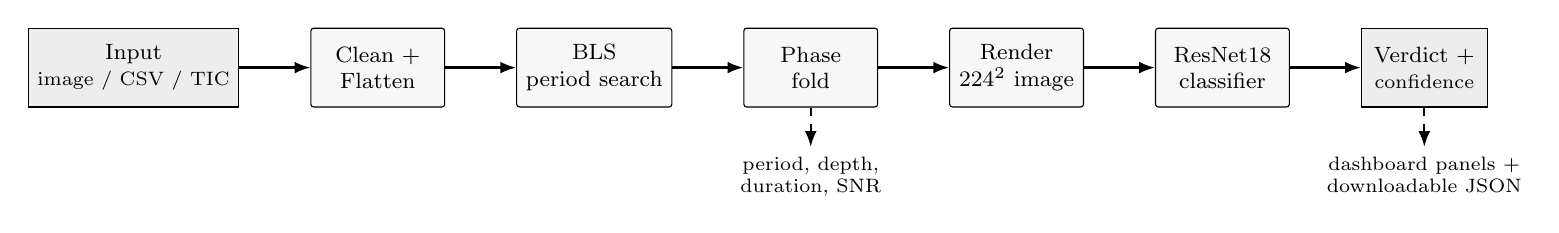
\begin{tikzpicture}[
  node distance=8mm and 9mm,
  box/.style={draw,rounded corners=1pt,minimum height=10mm,minimum width=17mm,
    align=center,font=\footnotesize,fill=gray!6},
  io/.style={draw,minimum height=10mm,minimum width=16mm,align=center,
    font=\footnotesize,fill=gray!14},
  arr/.style={-{Latex[length=2mm]},thick}
]
\node[io] (in) {Input\\\scriptsize image / CSV / TIC};
\node[box,right=of in] (clean) {Clean +\\Flatten};
\node[box,right=of clean] (bls) {BLS\\period search};
\node[box,right=of bls] (fold) {Phase\\fold};
\node[box,right=of fold] (render) {Render\\$224^2$ image};
\node[box,right=of render] (cnn) {ResNet18\\classifier};
\node[io,right=of cnn] (out) {Verdict +\\\scriptsize confidence};

\draw[arr] (in) -- (clean);
\draw[arr] (clean) -- (bls);
\draw[arr] (bls) -- (fold);
\draw[arr] (fold) -- (render);
\draw[arr] (render) -- (cnn);
\draw[arr] (cnn) -- (out);

\node[below=5mm of fold,font=\scriptsize,align=center] (params)
  {period, depth,\\duration, SNR};
\draw[arr,dashed] (fold) -- (params);
\node[below=5mm of out,font=\scriptsize,align=center] (dash)
  {dashboard panels +\\downloadable JSON};
\draw[arr,dashed] (out) -- (dash);
\end{tikzpicture}
\caption{End-to-end TESSNet pipeline. An input (a pre-rendered image, a raw
\code{time,flux} CSV, or a TESS Input Catalog identifier) is reduced through
cleaning, detrending, BLS period search, phase folding, and rasterization, then
classified by a fine-tuned ResNet18. Physical parameters and downsampled series
populate the dashboard; results are exportable as JSON. The image input enters the
pipeline directly at the classifier.}
\label{fig:pipeline}
\end{figure*}

\subsection{Overview}
The application is a Python/Flask service backed by PyTorch~\cite{paszke2019} for
inference and the Lightkurve/Astropy stack for reduction. A single-page front end
(HTML, CSS, and vanilla JavaScript with Chart.js for plotting) renders a
mission-control dashboard. The end-to-end flow is shown in
Figure~\ref{fig:pipeline}.

Three input modalities are supported, summarized in Table~\ref{tab:modes}. The
\emph{image} mode classifies a pre-rendered fold directly; the \emph{CSV} and
\emph{TIC} modes run the full reduction pipeline server-side and then repopulate
every dashboard panel (raw curve, denoised curve, transit-probability trace, and
phase fold) from the real data. The corresponding HTTP endpoints are listed in
Table~\ref{tab:api}.

\begin{table}[t]
\centering
\caption{Input modalities.}
\label{tab:modes}
\small
\begin{tabular}{@{}p{0.13\columnwidth}p{0.34\columnwidth}p{0.40\columnwidth}@{}}
\toprule
\textbf{Mode} & \textbf{Input} & \textbf{Action} \\
\midrule
Image & phase-folded PNG & classify directly \\
CSV   & \code{time,flux} file & full pipeline + classify \\
TIC   & TESS catalog ID & fetch from MAST, full pipeline \\
\bottomrule
\end{tabular}
\end{table}

\begin{table}[t]
\centering
\caption{HTTP API.}
\label{tab:api}
\small
\begin{tabular}{@{}llp{0.40\columnwidth}@{}}
\toprule
\textbf{Method} & \textbf{Route} & \textbf{Purpose} \\
\midrule
GET  & \code{/} & dashboard \\
GET  & \code{/api/model-status} & readiness + class labels \\
POST & \code{/predict} & classify one image \\
POST & \code{/analyze/csv} & full pipeline on a CSV \\
POST & \code{/analyze/tic} & fetch + full pipeline by TIC \\
\bottomrule
\end{tabular}
\end{table}

\subsection{Inference Service}
The model is loaded \emph{lazily} on first use rather than at process start. This
keeps the index route lightweight: readiness is reported by checking for the
presence of dependencies and the checkpoint file without importing the heavy
PyTorch stack, so a memory- or time-constrained host does not stall or get killed
during boot. The first classification request triggers a one-time construction of
the network and load of the weights.

\subsection{Batch Processing}
Each modality accepts \emph{multiple} inputs: several image or CSV files, or a list
of TIC identifiers. Items are processed \emph{sequentially} on the client, which
issues one request per item to the corresponding endpoint. Sequential execution is
a deliberate choice: BLS searches and MAST downloads are individually expensive,
and serial processing both bounds server load and yields a natural, honest
progress signal. A progress bar advances as each item completes, the dashboard
updates live with each result, and a scrollable per-item list records the verdict,
recovered period, and confidence for every target. Any single failure is recorded
inline and does not abort the batch.

\subsection{Result Export}
All results from a run---single or batch---are exportable as one JSON document.
We chose JSON because the output is heterogeneous: scalar parameters, a categorical
classification with per-class probabilities, and several time series of differing
lengths cannot be represented cleanly in a single flat CSV, whereas JSON captures
them losslessly and is trivially machine-readable. The export records, per item,
the source, classification, recovered parameters, and the (display-downsampled)
series, with an explicit note that the parameters and classification are computed
on the full-resolution light curve. Listing~\ref{lst:json} sketches the schema.

\begin{lstlisting}[caption={Abbreviated result-export schema.},label={lst:json}]
{
  "count": 3, "succeeded": 3, "failed": 0,
  "results": [
    {
      "source": "TIC 25155310",
      "ok": true,
      "classification": {
        "predicted_label": "Planetary Transit",
        "confidence": 0.97,
        "transit_detected": true,
        "probabilities": [ ... ]
      },
      "parameters": {
        "period_days": 10.02,
        "depth_pct": 1.21,
        "duration_hours": 2.71,
        "snr": 12.4
      },
      "series": { "raw": [...], "folded": [...] }
    }
  ]
}
\end{lstlisting}

\subsection{Visualization and Design}
The dashboard presents the workflow as a fixed, single-screen grid of panels: the
noisy input curve, a diagram of the AI pipeline, the denoised curve, the
transit-probability trace, and a detection summary with a phase-folded plot and the
rendered model-input image. Every panel offers a contextual help explainer and a
full-screen expansion with extended reference material. The visual language is a
documented dark design system---greyscale with a single electric-blue accent,
square corners, restrained motion, and an animated splash screen---intended to
read as an operations console rather than a generic form.

% ============================================================
\section{Implementation and Robustness}
Several engineering measures were necessary to make the service correct and stable
under realistic, concurrent deployment.

\textbf{Thread-safe rendering.} Image rendering uses Matplotlib's object-oriented
\code{Figure}/\code{Agg} API rather than the stateful \code{pyplot} interface.
Under a threaded WSGI worker, two concurrent reduction requests sharing
\code{pyplot}'s global figure registry could corrupt state; standalone figures
eliminate the shared state. The non-interactive \code{Agg} backend is forced so the
process never attempts to open a display.

\textbf{Concurrency-safe model loading.} Lazy initialization is guarded by a lock
with double-checked locking, so racing first-requests cannot redundantly build the
network or load the ${\sim}45$\,MB checkpoint twice.

\textbf{Input hardening.} Uploaded images with transparency are composited onto a
white background before conversion to RGB, matching the white-background training
distribution; a naive RGB conversion would render transparent regions black and
degrade predictions. Opaque library failures in the reduction stage (too-short
baseline, sparse sampling, periodogram errors, network failures during a MAST
fetch) are caught and surfaced as concise, human-readable messages.

\textbf{Graceful degradation.} If the plotting library fails to load on the client,
the interface degrades to a usable, no-op state rather than blanking. Heavy
dependencies are optional at the feature level: the image-classification mode
functions even where the full reduction stack is unavailable.

\textbf{Deployment footprint.} The service installs CPU-only PyTorch wheels to
avoid the multi-gigabyte CUDA build, and binds to a host-injected port for
platform port detection. A production configuration runs a small number of worker
processes and threads with generous request timeouts to accommodate slow BLS
searches and MAST downloads.

% ============================================================
\section{Functional Validation}
Because a large, vetted classifier benchmark is outside the present scope, we
validate the \emph{reduction stage}---the component that produces the model input
and the reported physical parameters---through injection--recovery experiments.
We generate synthetic light curves over a $27$-day baseline at ${\sim}0.01$-day
cadence, inject box-shaped transits of known period, depth, and duration, add
Gaussian noise, and scale to arbitrary detector units. Each synthetic curve is
passed through the live \code{/analyze/csv} endpoint.

\begin{table}[t]
\centering
\caption{Injection--recovery on synthetic transits. Periods are recovered exactly
to the $0.01$-day search-grid resolution. Recovered depth is a slight
underestimate of the injected value, consistent with detrending and finite
cadence. SNR is high because the injected noise is small.}
\label{tab:inj}
\small
\begin{tabular}{@{}cccccc@{}}
\toprule
$P_{\mathrm{inj}}$ & $P_{\mathrm{rec}}$ & $\delta_{\mathrm{inj}}$ &
$\delta_{\mathrm{rec}}$ & dur. & SNR \\
(d) & (d) & (\%) & (\%) & (h) & \\
\midrule
3.2 & 3.2 & 1.0 & 0.93 & 2.4 & 42.0 \\
4.5 & 4.5 & 1.2 & 0.97 & 3.6 & 46.6 \\
6.3 & 6.3 & 1.3 & 1.06 & 3.6 & 45.6 \\
\bottomrule
\end{tabular}
\end{table}

Table~\ref{tab:inj} reports representative results. In every case the BLS stage
recovers the injected period \emph{exactly} to the grid resolution; additional
injections at $3.7$, $5.5$, and $8.1$~days were likewise recovered exactly. The
recovered depth is consistently a small underestimate of the injected value, an
expected consequence of detrending and finite-cadence smoothing of the transit
shoulders. We additionally verified that transparent-background and
white-background renderings of the same scatter pattern yield identical
classifications (validating the input-compositing fix), that probabilities sum to
unity, and that concurrent reduction requests complete without error under the
thread-safe renderer and locked loader. These checks confirm that the system
produces correct, reproducible reductions end-to-end.

% ============================================================
\section{Limitations}
We are explicit about the prototype's boundaries. \textbf{(i)~Training data.} The
curated training set is small and dominated by a randomly-sampled noise class; the
shipped checkpoint is binary, and a planned eclipsing-binary class did not survive
into the final model. \textbf{(ii)~Classifier evaluation.} We do not report
precision, recall, or AUC, because doing so credibly requires a large, vetted
benchmark (for example, TESS Objects of Interest cross-matched with confirmed
eclipsing-binary catalogs); we deliberately avoid quoting unvalidated accuracy
figures. \textbf{(iii)~Image formulation.} Rendering the fold as an image discards
explicit per-cadence uncertainty and temporal ordering that 1D approaches retain.
\textbf{(iv)~Distribution sensitivity.} Because the model keys on a specific visual
style (black scatter on white), inputs that deviate stylistically must be rendered
consistently. \textbf{(v)~Transit-probability trace.} For real data this trace is
an ephemeris-derived in-transit indicator, not a learned per-cadence posterior.

% ============================================================
\section{Future Work}
Natural next steps include: scaling and balancing the training set with confirmed
TESS/Kepler transits and labeled false positives (eclipsing binaries, pulsators,
systematics); a rigorous benchmark reporting precision/recall and reliability
curves; multi-class extension (planet / eclipsing binary / variable / noise) to
exploit the morphological distinctions the dashboard already explains; calibrating
confidence scores for triage; and incorporating complementary vetting tests (odd--
even depth comparison, secondary-eclipse search, and centroid-shift analysis) as
additional model inputs or post-hoc filters. On the systems side, an
asynchronous job queue would allow large catalog batches to run server-side with
resumable progress.

% ============================================================
\section{Conclusion}
We presented TESSNet, an end-to-end system for exoplanet transit detection that
couples a classical BLS reduction pipeline with an image-based ResNet18 classifier
and wraps both in an interactive, deployable dashboard supporting single and batch
analysis across three input modalities. The contribution is as much architectural
as algorithmic: a faithful, robust path from raw flux---or a bare catalog
identifier---to a vetted, explainable, exportable candidate, engineered to run
correctly under concurrent, resource-constrained conditions. Injection--recovery
experiments confirm the correctness of the reduction stage, and the design lays a
clean foundation for the larger-scale classifier evaluation we identify as the
primary next step.

% ============================================================
\section*{Acknowledgments}
This work was developed for the ISRO Bharatiya Antariksh Hackathon (BAH) 2026. We
thank the Lightkurve, Astropy, and PyTorch communities, and the NASA MAST archive,
whose open tools and data underpin this system.

% ============================================================
\begin{thebibliography}{99}
\small
\bibitem{borucki2010} W.~J. Borucki et al., ``Kepler Planet-Detection Mission:
  Introduction and First Results,'' \emph{Science}, vol.~327, no.~5968, pp.~977--980,
  2010.
\bibitem{ricker2015} G.~R. Ricker et al., ``Transiting Exoplanet Survey Satellite
  (TESS),'' \emph{J. Astron. Telesc. Instrum. Syst.}, vol.~1, no.~1, 014003, 2015.
\bibitem{kovacs2002} G.~Kov\'acs, S.~Zucker, and T.~Mazeh, ``A box-fitting algorithm
  in the search for periodic transits,'' \emph{Astron. Astrophys.}, vol.~391,
  pp.~369--377, 2002.
\bibitem{shallue2018} C.~J. Shallue and A.~Vanderburg, ``Identifying Exoplanets with
  Deep Learning: A Five-planet Resonant Chain around Kepler-80 and an Eighth Planet
  around Kepler-90,'' \emph{Astron. J.}, vol.~155, no.~2, 94, 2018.
\bibitem{ansdell2018} M.~Ansdell et al., ``Scientific Domain Knowledge Improves
  Exoplanet Transit Classification with Deep Learning,'' \emph{Astrophys. J. Lett.},
  vol.~869, no.~1, L7, 2018.
\bibitem{he2016} K.~He, X.~Zhang, S.~Ren, and J.~Sun, ``Deep Residual Learning for
  Image Recognition,'' in \emph{Proc. IEEE Conf. Computer Vision and Pattern
  Recognition (CVPR)}, 2016, pp.~770--778.
\bibitem{deng2009} J.~Deng et al., ``ImageNet: A Large-Scale Hierarchical Image
  Database,'' in \emph{Proc. IEEE CVPR}, 2009, pp.~248--255.
\bibitem{lightkurve2018} Lightkurve Collaboration, ``Lightkurve: Kepler and TESS
  time series analysis in Python,'' Astrophysics Source Code Library, ascl:1812.013,
  2018.
\bibitem{astropy2018} Astropy Collaboration, ``The Astropy Project: Building an
  Open-science Project\ldots,'' \emph{Astron. J.}, vol.~156, no.~3, 123, 2018.
\bibitem{paszke2019} A.~Paszke et al., ``PyTorch: An Imperative Style,
  High-Performance Deep Learning Library,'' in \emph{Adv. Neural Inf. Process. Syst.
  (NeurIPS)}, 2019, pp.~8024--8035.
\end{thebibliography}

\end{document}
